\documentclass[11pt]{article}

\usepackage[a4paper, total={16cm, 24cm}]{geometry}
\usepackage[portuguese]{babel}
\usepackage[utf8]{inputenc}
\usepackage{graphicx}
\usepackage{amsmath}
\usepackage{tikz}
    \usetikzlibrary{shadows}
\usepackage{booktabs}
\usepackage[colorlinks=true]{hyperref}
\usepackage{listings}
    \renewcommand\lstlistingname{Listagem}
    \lstset{numbers=left, numberstyle=\tiny, numbersep=5pt, basicstyle=\footnotesize\ttfamily, frame=tb,rulesepcolor=\color{gray}, breaklines=true}
\usepackage{blindtext}

% -------------------------------------------------------------------------------------------
\title
{
    
\includegraphics[width=0.4\textwidth]{imgs/university.png}
    \\[0.1cm]
    \textbf{2º Trabalho - Hard Weeks} \\
    Estrutura de Dados e Algoritmos II
}

\author
{
    \textbf{Professora:} Vasco Pedro \\
    \textbf{Realizado por:} Filipe Alfaiate (43315), Miguel de Carvalho (43108) 
}
\date{\today}

% -------------------------------------------------------------------------------------------
%                                Body                                                       %
% -------------------------------------------------------------------------------------------

\begin{document}
\maketitle

% -------------------------------------------------------------------------------------------
\section{Algoritmo}

\hspace{0,5cm}O nosso algoritmo consiste na utilização de um \textbf{grafo orientado acíclico}
onde os vértices representam tarefas e o arco que vai da \verb|tarefa1| à \verb|tarefa2| corresponde
a uma dependência da \verb|tarefa2| face à \verb|tarefa1|, ou seja, a \verb|tarefa1| tem que ser
concluída antes da \verb|tarefa2| (\verb|tarefa1 < tarefa2|).

A utilização deste \textbf{algoritmo} baseia-se num planeamento de projeto que dado um \textbf{número de
tarefas} mostra o \textbf{maior número de tarefas} numa única semana e o \textbf{número de semanas más}.

% -------------------------------------------------------------------------------------------
\section{Análise do Grafo}

\hspace{0,5cm}Utilizando a \textbf{ordenação topoplógica}, a construção do \textbf{grafo} (exemplo do enunciado)
seria:

\verb|0 < 5, 0 < 6, 1 < 0, 1 < 6, 1 < 7, 7 < 2, 5 < 8,|

\verb|8 < 9, 10 < 3, 8 < 6, 4 < 10, 7 < 9, 4 < 11, 6 < 7|

\begin{center}
    \begin{figure}[h!]
        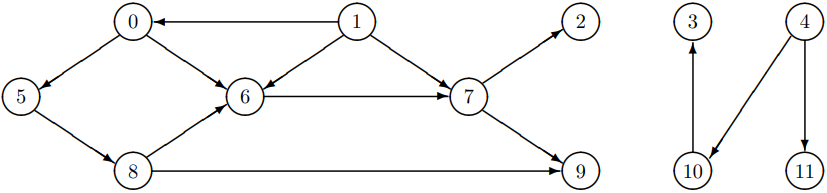
\includegraphics[width=0.8\textwidth]{imgs/grafo.png}
        \caption{Grafo inicial}
        \label{fig:grafoIni}
    \end{figure}
\end{center}

Em seguida percorremos todos os \textbf{nós} para verificar quais não apresentam antecedentes,
colocando os mesmos numa \textbf{fila}.

Como estamos a fazer uma pesquisa semanal (pesquisa em largura), as novas tarefas inseridas nunca terão
uma semana menor que as semanas que estão à sua frente na fila. Isto significa que quando \textbf{visualizamos a
primeira tarefa da fila} vamos verificar que todas as \textbf{tarefas restantes na fila} serão da mesma semana,
o que indica o número de tarefas que terão de ser realizadas nessa semana. Apenas quando esse grupo de
tarefas sair da fila, poderemos iniciar de novo este processo. 

Posteriormente retiramos o primeiro elemento da fila e procuramos os seus \textbf{precedentes}, atualizando a
semana para a semana deste antecedente e decrementamos o número de antecedentes, acrescentando esta tarefa à
\textbf{fila} se já não tiver \textbf{tarefas que a antecedam}.

Este processo é repetido até a \textbf{fila ficar vazia}.

\begin{center}
    \begin{figure}[h!]
        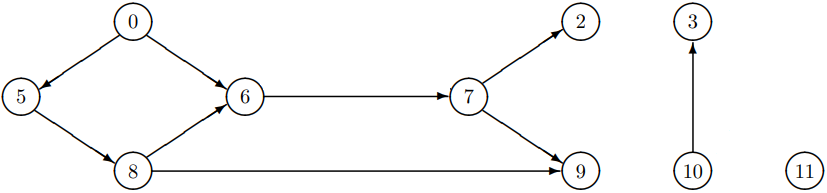
\includegraphics[width=0.8\textwidth]{imgs/grafo1.png}
        \caption{Grafo sem as tarefas da semana 1}
        \label{fig:grafo1}
    \end{figure}
    \begin{figure}[h!]
        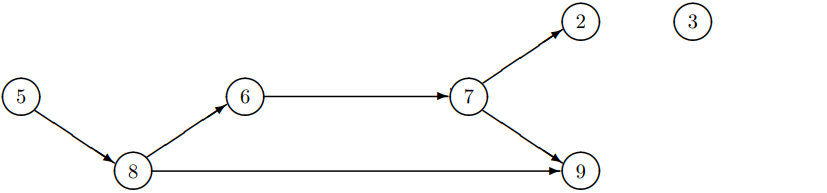
\includegraphics[width=0.8\textwidth]{imgs/grafo2.png}
        \caption{Grafo sem as tarefas da semana 2}
        \label{fig:grafo2}
    \end{figure}
    \begin{figure}[h!]
        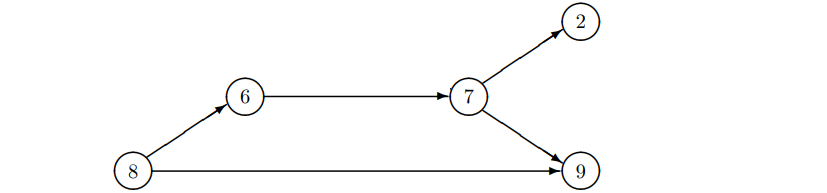
\includegraphics[width=0.8\textwidth]{imgs/grafo3.png}
        \caption{Grafo sem as tarefas da semana 3}
        \label{fig:grafo3}
    \end{figure}
    \begin{figure}[h!]
        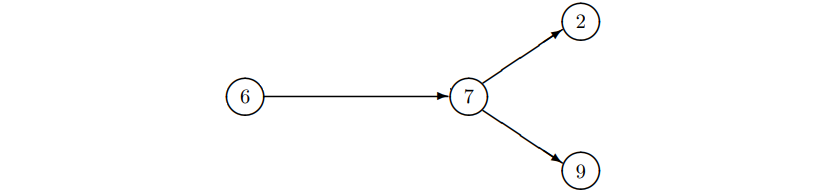
\includegraphics[width=0.8\textwidth]{imgs/grafo4.png}
        \caption{Grafo sem as tarefas da semana 4}
        \label{fig:grafo4}
    \end{figure}
    \begin{figure}[h!]
        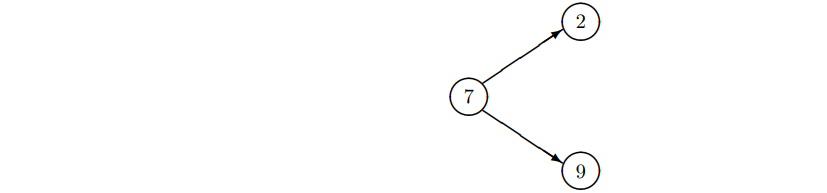
\includegraphics[width=0.8\textwidth]{imgs/grafo5.png}
        \caption{Grafo sem as tarefas da semana 5}
        \label{fig:grafo5}
    \end{figure}
    \begin{figure}[h!]
        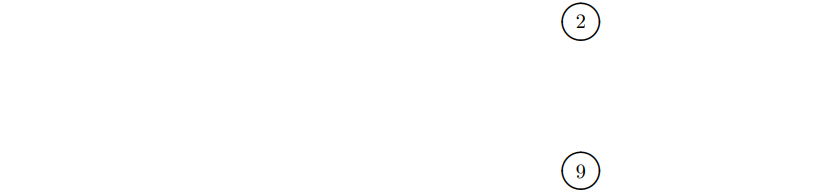
\includegraphics[width=0.8\textwidth]{imgs/grafo6.png}
        \caption{Grafo sem as tarefas da semana 6}
        \label{fig:grafo6}
    \end{figure}
\end{center}

% -------------------------------------------------------------------------------------------
\section{Complexidade}
\subsection{Temporal}

\hspace{0,5cm}Começámos por proceder à leitura de uma \verb|string| com 3 números, \textbf{número de tarefas},
\textbf{precedência direta entre tarefas} e o \textbf{limite usado para definir uma semana má}, respetivamente,
o que origina uma complexidade constane \verb|O(1)|.

Procedeu-se à verificação dos inputs referidos no parágrafo anterior estarem dentro dos limites permitidos do
programa, demorando um tempo constante \verb|O(1)| para cada condição.

De seguida declarámos um vetor de listas e uma fila, que apresenta um custo constante \verb|O(1)|.

Posteriormente iniciámos um ciclo para percorrer todos os nós inicializando-os, dando valores e colocando-os numa
lista na posição do seu valor, o que tem custo constante, mas como estamos a percorrer todos os nós teremos um
custo linear em relação ao número de nós, \verb|O(V)|, sendo \verb|V| o número de nós.

Além disso, teremos um ciclo para criar o grafo, ou seja, estabelecer adjacências entre os 
\textbf{nós}, onde procedemos à leitura de uma string com dois números, representando o arco (t1,t2) que corresponde
a \verb|t1 -> t2|. É criada essa ligação e \verb|t2| incrementa o antecedente, todas estas operações apresentam
um custo constante \verb|O(1)|, mas como temos que percorrer todas as \textbf{precedências diretas entre
tarefas} a complexidade é \verb|O(E)| onde \verb|E| é o número de arcos.

Também de forma cíclica percorremos todos os \textbf{nós}, após estes terem sido relacionados entre eles, para
achar quais os nós sem antecedentes,colocando os mesmos numa \textbf{fila}, o que nos dá um complexidade
linear \verb|O(V)| onde \verb|V| é o número de nós.

Foram incializidas três variavéis que servem de contadores e apresentam custo constante \verb|O(1)|.

Por fim percorremos a fila até esta se encontrar vazia, como cada \textbf{nó} só vai aparecer uma única e
exclusiva vez na \textbf{fila} iremos ter uma complexidade \verb|O(V)|, sendo \verb|V| o número de
\textbf{nós}. A cada remoção feita da fila serão realizadas várias afetações e condições, todas elas
constantes \verb|O(1)|, excepto a pesquisa de \textbf{nós adjacentes} tem custo \verb|O(E)|, onde
\verb|E| é o \textbf{número de arestas}. Quando a fila estiver vazia, podemos afirmar que o custo é
de \verb|O(V+E)|, onde \verb|V| é o \textbf{número de nós} e \verb|E| é o \textbf{número de arcos}.

\begin{center}
    \textbf{O(1) + O(1) + O(1) + O(V) + O(E) + O(V) + O(V+E) = O(V+E)}
\end{center}

\subsection{Espacial}

\hspace{0,5cm}Durante a inicialização do vetor de listas teremos que reservar um espaço em memória onde
serão guardados as \verb|V| cabeças da lista, o que irá ocupar em memória \verb|O(V)|, onde
\verb|V| é o número de nós do grafo.

Ao inicializar a fila vamos criar um \textbf{nó inicial} o que irá ocupar um espaço em memória de \verb|O(1)|

Quando são criados os \textbf{nós do grafo} terá de ser guardado individualmente originando assim uma
complexidade espacial de \verb|O(V)|, onde \verb|V| é o número de \textbf{nós do grafo}. 
De seguida guardamos os mesmos na cabeça da lista da sua posição.

Quando adicionamos as adjacências pretendidas em cada posição do \textbf{vetor de listas} iremos ter uma
complexidade de \verb|O(V+E)|, onde \verb|V| é o \textbf{número de nós} e \verb|E| é \textbf{número de
arestas do grafo}.

Para finalizar a \textbf{complexidade espacial}, quando manipulamos a fila, adicionamos e removemos \textbf{nós}
ao longo dessa mesma manipulação, mas tendo em conta o pior caso a fila poderá conter todos os \textbf{nós
do grafo} o que irá originar uma \textbf{complexidade espacial} de \verb|O(V)|, onde \verb|V| é o
\textbf{número de nós}.

\begin{center}
    \textbf{O(V) + O(1) + O(V) + O(V+E) + O(V) = O(V+E)}
\end{center}

% -------------------------------------------------------------------------------------------
\section{Comentários Adicionais}

\hspace{0,5cm}Na realização deste trabalho foi usado uma \textbf{disciplina de fila}, pois era a única
que mantinha uma ordem sequêncial em relação ao número da semana, mas qualquer outra disciplina
serviria para o mesmo fim, apenas não de uma forma tão direta e possivelmente com \textbf{maior custo
temporal ou espacial}.

Uma outra observação a ter em conta foi a escolha de um \textbf{vetor de listas de adjacências}, em vez
de uma \textbf{matriz de adjacências}. Esta escolha não foi baseada só em termos de \textbf{complexidade
temporal/espacial} mas também na forma como a informação é guardada em memória, pois numa \textbf{matriz
de adjacências} a informação teria de ser guardada sequencialmente arranjando um espaço $\verb|V|^{2}$,
onde \verb|V| é o \textbf{número de nós do grafo}, e um \textbf{vetor de listas de adjacências} apenas
teria que guardar sequencialmente o vetor onde se encontra a cabeça da lista e essa de seguida tem um
apontador para a posição em memória do próximo elemento da lista, isto significa que esse \textbf{nó em
memória} poderá estar em qualquer parte da memória facilitando a sua \textbf{organização em memória}.
% -------------------------------------------------------------------------------------------
\end{document}